\section{Experiments}
\label{sec:experiments}

% === Other stuff.

In this section, we empirically evaluate our approach on three tasks. 
While the on-the-job setting we propose is targeted at scenarios where there is
no data to begin with, we use existing labeled datasets (\reftab{dataset}) to have a gold standard.
%empirically evaluate the performance of our system relative to baselines.

\paragraph{Baselines.}
We evaluated the following four methods on each dataset:
\begin{enumerate}
  \item {\bf Human n-query}: The majority vote of $n$ human crowd workers was used as a prediction.
  \item {\bf Online learning}:
    Uses a classifier that trains on the gold output for all examples seen so
    far and then returns the MLE as a prediction.
    This is the best possible offline system: it sees perfect information about all the data seen so far, but can not query the crowd while making a prediction.
  \item {\bf Threshold baseline}: Uses the following heuristic:
    For each label, $y_i$, we ask for $m$ queries such that $(1 - \p(y_i\given \bx))\times 0.3^m \ge 0.98$. % \footnote{We found $0.88$ to give the best results on our datasets.}
    Instead of computing the expected marginals over the responses to queries in flight,
    we simply count the in-flight requests for a given variable, and reduces
    the uncertainty on that variable by a factor of $0.3$. The system continues
    launching requests until the threshold (adjusted by number of queries in
    flight) is crossed. Predictions are made using MLE on the model given
    responses.
    The baseline does not reason about time and makes all its queries at the very beginning.
  \item {\bf LENSE:} Our full system as described in \refsec{model}.
\end{enumerate}

% === Figures
\begin{table}[t]
  \begin{tabular}{l p{0.35\textwidth} p{0.35\textwidth} r r r}
    {\bf Dataset (Examples)} & {\bf Task and notes} & {\bf Features} \\ \hline
  {\bf NER (657)}     & 
    We evaluate on the CoNLL-2003 NER task\tablefootnote{\href{http://www.cnts.ua.ac.be/conll2003/ner/}{http://www.cnts.ua.ac.be/conll2003/ner/}}, a sequence labeling problem over English sentences. 
    We only consider the four tags corresponding to persons, locations, organizations or none\tablefootnote{
    The original also includes a fifth tag for miscellaneous, however the definition for miscellaneos is complex, making it very difficult for non-expert crowd workers to provide accurate labels.}.
    &
    We used standard features~\cite{finkel2005incorporating}: the current word, current lemma, previous and next lemmas, lemmas in a window of size three to the left and right, word shape and word prefix and suffixes, as well as word embeddings. \\
  {\bf Sentiment (1800)} & 
    We evaluate on a subset of the IMDB sentiment dataset \cite{maas2011imdb} that consists of 2000 polar movie reviews; the goal is binary classification of documents into classes $\textsc{pos}$ and $\textsc{neg}$. 
    &
    We used two feature sets, the first (\textsc{unigrams}) containing only word unigrams, and the second (\textsc{rnn}) that also contains sentence vector embeddings from~\cite{socher2013recursive}.
    \\
  {\bf Face (1784)} & 
  We evaluate on a celebrity face classification task \cite{kumar2009attribute}. Each image must be labeled as one of the following four choices: Andersen Cooper, Daniel Craig, Scarlet Johansson or Miley Cyrus.
    &
    We used the last layer of a 11-layer AlexNet~\cite{krizhevsky2012imagenet} trained on ImageNet as input feature embeddings, though we leave back-propagating into the net to future work.
\end{tabular}
  \caption{Datasets used in this chapter and number of examples we evaluate on.}
\label{tbl:dataset}
\end{table}


% To initialize parameters for the model-based methods, we used a burn-in period of 40 examples during which everything was labeled. We used those responses to train initial parameters for the prediction model $\theta$, response model $\beta$ and delay model $\Gamma$.
% We do not update parameters for the delay and response models online.

\paragraph{Implementation and crowdsourcing setup.}
We implemented the retainer model of~\cite{bernstein2011crowds} on Amazon Mechanical Turk to create a ``pool'' of crowd workers that could respond to queries in real-time.
The workers were given a short tutorial on each task before joining the pool to minimize systematic errors caused by misunderstanding the task.
We paid workers \$1.00 to join the retainer pool and an additional \$0.01 per query (for NER, since response times were much faster, we paid \$0.005 per query).
Worker response times were generally in the range of 0.5--2 seconds for NER, 10--15 seconds for Sentiment, and 1--4 seconds for Faces.

When running experiments, we found that the results varied based on the current worker quality. %, fluctuating on the NER task between 87 and 96 F1, depending on workers.
To control for variance in worker quality across our evaluations of the different methods, we collected 5 worker responses and their delays on each label ahead of time\footnote{These datasets are available in the code repository for this paper}.
During simulation we sample the worker responses and delays without replacement from this frozen pool of worker responses.

\begin{table}[t]
%% NER 
\centering
\begin{tabular}{l r r r r r r}
  \toprule
      \textbf{System} & \textbf{Delay/tok} & \textbf{Qs/tok} & \textbf{PER F$_1$} & \textbf{LOC F$_1$} & \textbf{ORG F$_1$} & \textbf{F$_1$}
    \\ \midrule
    1-vote & 467 ms & 1.0 & 90.2 & 78.8 & 71.5 & 80.2 \\
    3-vote & 750 ms & 3.0 & 93.6 & 85.1 & 74.5 & 85.4 \\
    5-vote & 1350 ms & 5.0 & \textbf{95.5} & 87.7 & 78.7 & 87.3  \\ \midrule
    Online & n/a & n/a & 56.9 & 74.6 & 51.4 & 60.9 \\
    Threshold & 414 ms & 0.61 & 95.2 & \textbf{89.8} & 79.8 & 88.3 \\
    \textbf{LENSE} & \textbf{267 ms} & \textbf{0.45} & 95.2 & 89.7 & \textbf{81.7} & \textbf{88.8}  \\
    \bottomrule
\end{tabular}
\caption[Results on NER]{\label{tbl:results-ner} Results on the NER task comparing latencies, queries per token (Qs/tok)
and \fone{}.}
\end{table}

\begin{table}[t]
  \centering
\begin{tabular}{l r r r}
  \toprule
      \textbf{System} & \textbf{Latency} & \textbf{Qs/ex} & \textbf{Acc.} 
    \\ \midrule
    1-vote & 1216 ms & 1.0 & 93.6 \\ %\hline
    3-vote & 1782 ms & 3.0 & 99.1 \\ %\hline
    5-vote & 2103 ms & 5.0 & 99.8 \\ \midrule
    Online & n/a & n/a & 79.9 \\    %\hline
    Threshold & 1680 ms & 2.66 & 93.5 \\ %\hline
    \textbf{LENSE} & 1590 ms & 2.37 & 99.2 \\   %\hline
    \bottomrule
\end{tabular}
\caption[Results on Face]{\label{tbl:results-face} Results on the Face task comparing latencies, queries per token (Qs/tok)
and accuracy.}
\end{table}

\begin{figure}[t]
\centering
  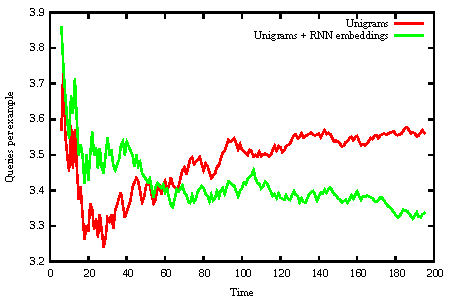
\includegraphics[width=0.6\textwidth]{figures/sentiment_cost_per_token_vs_time/cost_per_token_vs_time.pdf}
  \caption[Queries per example for LENSE on Sentiment.]{\label{fig:sentiment-tradeoff}Queries per example for LENSE on Sentiment. With simple \textsc{unigram} features, the model quickly learns it does not have the capacity to answer confidently and must query the crowd. With more complex \textsc{rnn} features, the model learns to be more confident and queries the crowd less over time.}
\end{figure}

\begin{table}[t]
  \centering
  \begin{tabular}{l r  r  r}
    \textbf{System} & \textbf{Latency} & \textbf{Qs/ex} & \textbf{Acc.} \\ \hline
    1-vote & 6.6 s & 1.00 & 89.2 \\ %\hline
    3-vote & 10.9 s & 3.00 & 95.8 \\ %\hline
    5-vote & 13.5 s & 5.00 & 98.7 \\ %\hline
    \multicolumn{4}{c}{\textsc{unigrams}} \\ \hline
    Online & n/a & n/a & 78.1 \\ %\hline
    Threshold & 10.9 s & 2.99 & 95.9 \\ %\hline
    \textbf{LENSE} & 11.7 s & 3.48 & 98.6 \\ %\hline
    \multicolumn{4}{c}{\textsc{rnn}} \\ \hline
    Online & n/a & n/a & 85.0 \\ %\hline
    Threshold & 11.0 s & 2.85 & 96.0 \\ %\hline
    \textbf{LENSE} & 11.0 s & 3.19 & 98.6 \\% \hline
\end{tabular}

  \caption[Results on the Sentiment task]{\label{tbl:sentiment-results}Results on the Sentiment task comparing latency, queries per example and accuracy.}
\end{table}

% DETAILS
% Anecdotally, we also report a range of results on 5 complete runs of our system using {\em real live crowd workers}, recruited at test time, over the first 150 sentences of our dataset. The results exhibit high variance based on worker quality.
%
%\begin{center}
%\begin{tabular}{ | r | r | r | r | r | }
%    \hline
%    Time/token & Requests/token & Precision & Recall & F1 \\ \hline
%    1444 ms - 3426 ms & 0.54 - 0.66 & 92.9 - 96.91 & 82.50 - 94.01 & 87.4 - 95.43 \\ \hline
%\end{tabular}
%\end{center}
%
%Filtering workers while running, or inferring separate error models for each worker, would clearly deliver substantial gains in reliability over a system that assumes uniform quality. We leave this to future work.

\paragraph{Summary of results.}
\reftab{results-ner}, \reftab{results-face} and \reftab{sentiment-results} summarize the performance of the methods on the three tasks.
On all three datasets, we found that on-the-job learning outperforms machine and human-only comparisons on both quality and cost. 
On NER, we achieve an \fone{} of $88.4\%$ at more than an order of magnitude
reduction on the cost of achieving comporable quality result using the 5-vote
approach. On Sentiment and Faces, we reduce costs for a comparable accuracy by
a factor of around 2.
For the latter two tasks, both on-the-job learning methods perform less well
than in NER.\@
We suspect this is due to the presence of a dominant class
(``none'') in NER that the model can very quickly learn to expend almost no
effort on.  LENSE outperforms the threshold baseline, supporting the importance
of Bayesian decision theory.

\begin{figure}[!p]
  \centering
  \begin{subfigure}[b]{0.8\textwidth}
  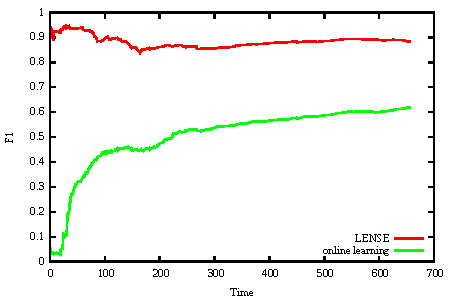
\includegraphics[width=\textwidth]{figures/ner_2_class/f1_plot/f1_vs_time.pdf}
\end{subfigure}

  \begin{subfigure}[b]{0.8\textwidth}
  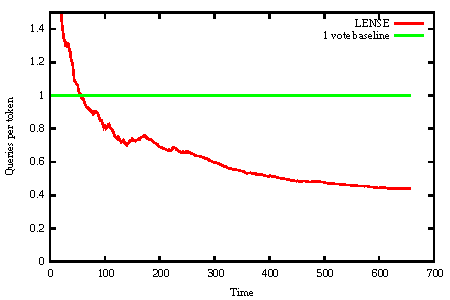
\includegraphics[width=\textwidth]{figures/ner_2_class/cost_plot/cost_vs_time.pdf}
  \end{subfigure}
  \caption[Comparing \fone{} and queries per token on the NER task over time.]{\label{fig:ner-f1} Comparing \fone{} and queries per token on the NER task over time. The left graph compares LENSE to online learning (which cannot query humans at test time). This highlights that LENSE maintains high \fone{} scores even with very small training set sizes, by falling back the crowd when it is unsure. The right graph compares query rate over time to 1-vote. This clearly shows that as the model learns, it needs to query the crowd less.}

\end{figure}

%\paragraph{Does the model respect accuracy preferences?} 
\reffig{ner-f1} tracks the performance and cost of LENSE over time on the NER task.
LENSE is not only able  to consistently outperform other baselines, but the cost of the system steadily reduces over time.
On the NER task, we find that LENSE is able to trade off time to produce more
accurate results than the 1-vote baseline with fewer queries by waiting for
responses before making another query.

% == DEV F1
%We also plot \fone{} on a held-out set: while we receive noisy and sparse supervision LENSE is able to train a classifier that generalizes well over time. 
%Compared to the offline baseline, which sees perfect labels on all examples, LENSE observed labels on only \ac{KEENON: fix this number: 600} words. For a comparable number of tokens, the offline baseline has an \fone of \ac{KEENON: fix: 63\%}.

% === Compare with threshold
%\paragraph{Why is the threshold system so much better on sentiment and faces?}
%LENSE exploits structure in the model when querying, and so outperforms the threshold in the presence of structure (see NER task results).
%However, when neither structure or time pressure is present, LENSE's only signal is the entropy of the prediction, and so the threshold is able to perform just as well, if not slightly better when the threshold is optimally set.

%We note that although our model is receiving supervisition signal at roughly 1/15 the rate of a fully observed online learning scenario\footnote{this calculation assumes ``fully observed'' is approximated by 3 human labels per example}, we track roughly parallel to the fully supervised line.

%\paragraph{In the limit, would LENSE still need crowd supervision?}
While on-the-job learning allows us to deploy quickly and ensure good results, we would like to eventually operate without crowd supervision.
%In order to do so, we must ensure that our model has the capacity to keep learning from the crowd.
\reffig{sentiment-tradeoff}, we show the number of queries per example on Sentiment with two different features sets, \textsc{unigrams} and \textsc{rnn} (as described in \reftab{dataset}).
With simpler features (\textsc{unigrams}),
the model saturates early and we will continue to need to query to the crowd to achieve our accuracy target (as specified by the loss function).
On the other hand, using richer features (\textsc{rnn}) the model is able to learn from the crowd and the amount of supervision needed reduces over time.
%This suggests that given a sufficiently rich model, costs can be brought to zero in the limit.
Note that even when the model capacity is limited, LENSE is able to guarantee a consistent, high level of performance.

\paragraph{Reproducibility.}
All code, data, and experiments for this paper are available on CodaLab at
{\small \url{https://www.codalab.org/worksheets/0x2ae89944846444539c2d08a0b7ff3f6f/}}.

% -- CUT
%\paragraph{When does LENSE query?}
%During the initial stages of learning for the NER task, LENSE made multiple queries on all tokens.
%After a few examples, though, LENSE focused its queries on unseen entity tokens.
%Consider the following example taken from our run logs: \textit{``U.S.\ says still committed to Cuba migration pacts''}.
%%For example, after seeing \ac{600} examples, 
%The model has already seen {\it U.S.\/} and predicts that it is a \scloc{} with 97\% probability.
%On the other hand, having never seen the token {\it Cuba\/} before, the model starts with a belief that {\it Cuba\/} is 59\% \scper, 37\% \scloc{} and 3\% \scnone.
%It immediately fires off two queries about {\it Cuba\/} and waits 4 seconds for both responses to return \scloc{}.
%The model now believes that {\it Cuba\/} is \scloc{} with 95\% probability and returns its prediction.
%This demonstrates that using the model allows LENSE to focus supervision to where it is needed.


% \paragraph{Are we learning a good model?}
% We receive very noisy and sparse supervision.
% Despite this, to reduce the costs in the future, our system must learn to generalize well.
% We refer to \reffig{ner-dev-f1}.
% We note that although our model is receiving supervisition signal at roughly 1/15 the rate of a fully observed online learning scenario\footnote{this calculation assumes ``fully observed'' is approximated by 3 human labels per example}, we track roughly parallel to the fully supervised line.

% Held out figure for space concerns.
%\begin{figure}[t]
%  \begin{centering}
%  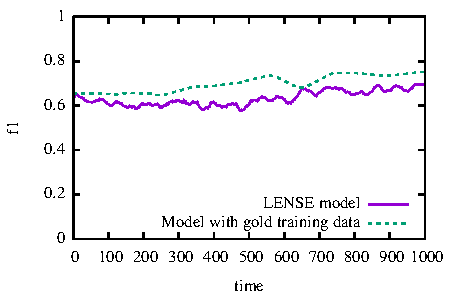
\includegraphics[width=1.0\textwidth]{figures/ner_2_class/machine_f1_plot/machine_f1_vs_time.pdf}
%  \end{centering}
%  \caption{A figure showing the relationship between the classifier we train, and one trained on gold labeled data. Evaluation is on a held out dev set. Note that our classifier learns more slowly because we are handing it a noisy approximation to train on, but the classifier narrows the gap as it gets more data.}
%\label{fig:ner-dev-f1}
%\end{figure}

